\chapter{Velocidad de reacción}\label{ch:g12:reaction-rates}

Una botella de leche olvidada en la encimera de la cocina se agria en un
par de días; en la nevera se conserva más de una semana. Un fuego
artificial \omterm{def:g4:what-a-fire-needs:burning}{arde} en una fracción de segundo, mientras que una estatua de
caliza de un parque urbano se desgasta a lo largo de siglos. Las
\omterm{def:g8:balanced-equations:equation}{ecuaciones ajustadas} y las \omterm{def:g10:reaction-progress-table:extent}{tablas de avance} dicen qué da una reacción y
cuánto; no dicen nada sobre su rapidez. En este capítulo medimos la
velocidad de las reacciones, buscamos lo que la controla y describimos la
forma más sencilla en que una reacción puede frenarse a medida que avanza.

\begin{recall}
La concentración de una disolución (\cref{ch:g10:concentration-and-dilution})
y el avance de una reacción (\cref{ch:g10:reaction-progress-table}). La
\omterm{def:g11:absorbance:absorbance}{absorbancia} de una disolución diluida es proporcional a la concentración
de la especie coloreada (\cref{ch:g11:absorbance}). Una \omterm{def:g11:titration:titration}{valoración} mide
la cantidad de una especie (\cref{ch:g11:titration}).
\end{recall}

\begin{omfigure}
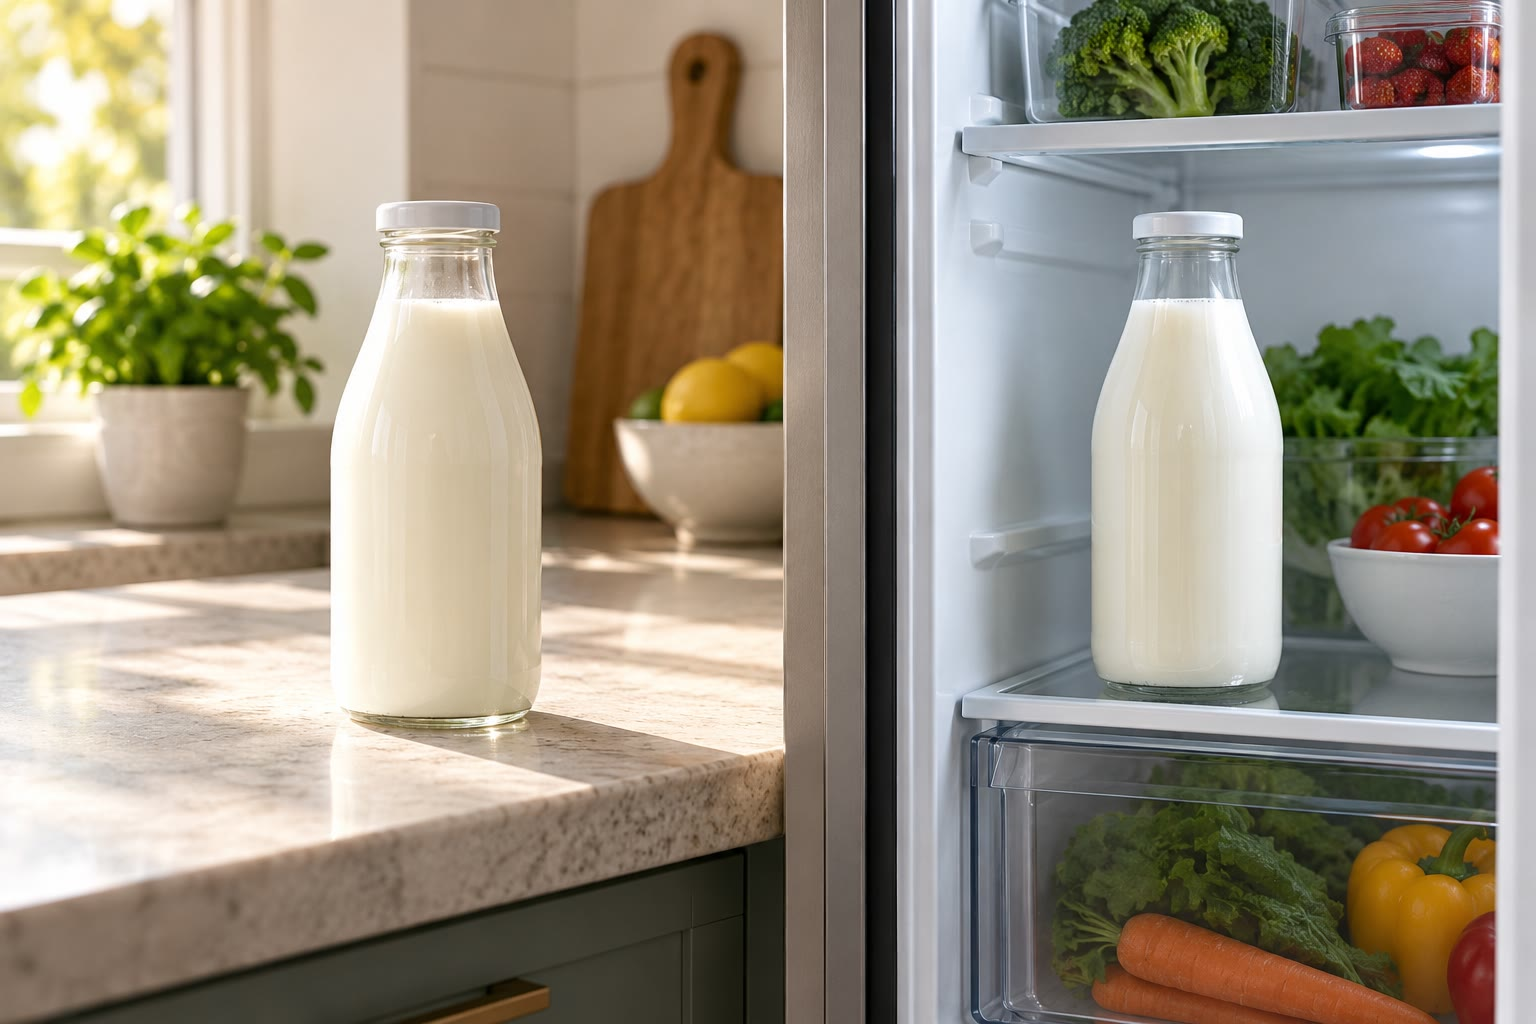
\includegraphics[width=0.48\linewidth]{images/book1/ai/g12-milk-counter-fridge.jpg}

{\small La misma leche, en la encimera y en la nevera: las reacciones que
la agrian son más lentas en frío.}
\end{omfigure}

\section{Seguir una reacción en el tiempo}

Algunas reacciones terminan en cuanto los \omterm{def:g7:chemical-reactions:reactant}{reactivos} se encuentran: la
\omterm{def:g9:ions:precipitate}{precipitación} del cloruro de plata, la reacción de un ácido con una base.
Otras tardan minutos, horas o años. Para estudiar una reacción lenta, los
químicos miden la concentración de un \omterm{def:g7:chemical-reactions:reactant}{reactivo} o de un producto a
intervalos regulares. Pueden
\begin{itemize}
  \item tomar pequeñas muestras, detener la reacción en cada una y
        valorarlas;
  \item medir la \omterm{def:g11:absorbance:absorbance}{absorbancia} de la disolución, cuando un \omterm{def:g7:chemical-reactions:reactant}{reactivo} o un
        producto es coloreado;
  \item medir la presión o el volumen de un gas desprendido, o la
        conductividad de una disolución cuyos \omterm{def:g9:ions:ion}{iones} cambian.
\end{itemize}

\begin{definition}[Bloqueo cinético]\label{def:g12:reaction-rates:quenching}
El \emph{bloqueo cinético}\index{bloqueo cinetico@bloqueo cinético} de una muestra consiste
en detener, o frenar muchísimo, la reacción que tiene lugar en ella en el
momento de tomarla, normalmente enfriándola de golpe y diluyéndola, para
poder medir su composición con calma.
\end{definition}

\begin{inthelab}[Bloquear una muestra]
Cada cinco minutos se toman con una pipeta \qty{10.0}{mL} de la \omterm{def:g6:pure-substances-and-mixtures:mixture}{mezcla} de
reacción y se vierten en un vaso de precipitados con unos \qty{40}{mL} de
agua helada. Diluida cinco veces y enfriada hasta cerca de
\qty{0}{\celsius}, la reacción se vuelve tan lenta que puede considerarse
detenida; después se valora la muestra. El instante de la muestra es el
momento en que se vierte en el agua helada, no el de la \omterm{def:g11:titration:titration}{valoración}.
\end{inthelab}

\begin{omfigure}
\begin{tikzpicture}[font=\small, scale=0.8]
  \pic[transform shape] at (0,0) {erlenmeyer={0.4}{orange!25}};
  \node[anchor=north, align=center] at (0,-0.15) {mezcla de\\ reacción};
  \pic[transform shape, rotate=-35] at (1.4,1.2) {pipette={0.6}{orange!25}};
  \draw[omProp, very thick, -{Stealth}] (1.6,0.8) -- (2.9,0.8);
  \node[anchor=south] at (2.25,0.85) {\qty{10.0}{mL}};
  \pic[transform shape] at (4,0) {beaker={0.55}{cyan!12}};
  \foreach \p in {(3.6,0.4),(4.2,0.6),(3.9,0.85),(4.4,0.3)}
    \draw[black!30, fill=white] \p ++(-0.1,-0.08) rectangle ++(0.2,0.16);
  \node[anchor=north, align=center] at (4,-0.15) {agua helada:\\ reacción detenida};
  \draw[omProp, very thick, -{Stealth}] (5.1,0.8) -- (6.4,0.8);
  \pic[transform shape] at (7.5,0) {erlenmeyer={0.35}{orange!12}};
  \pic[transform shape] at (7.5,2.75) {burette={0.7}{violet!45}};
  \node[anchor=north, align=center] at (7.5,-0.15) {valoración\\ de la muestra};
\end{tikzpicture}

{\small Seguir una reacción por muestreo: tomar una muestra, bloquearla y
medirla después con calma.}
\end{omfigure}

\section{Factores cinéticos}

\begin{definition}[Factor cinético]\label{def:g12:reaction-rates:kinetic-factor}
Un \emph{factor cinético}\index{factor cinetico@factor cinético} es una magnitud que
modifica la velocidad de una reacción sin cambiar lo que la reacción da:
la temperatura, las concentraciones de los \omterm{def:g7:chemical-reactions:reactant}{reactivos}, la superficie de
contacto entre \omterm{def:g7:chemical-reactions:reactant}{reactivos} en fases distintas y la presencia de un
catalizador (capítulo siguiente).
\end{definition}

\begin{proposition}[Más caliente, más concentrado, más fino: más rápido]\label{prop:g12:reaction-rates:factors}
En general, una reacción es más rápida cuando la temperatura es más
alta, cuando los \omterm{def:g7:chemical-reactions:reactant}{reactivos} están más concentrados y, en el caso de un
\omterm{def:g7:chemical-reactions:reactant}{reactivo} sólido, cuando está más finamente dividido.
\end{proposition}

\begin{proof}
Se admite, con una imagen: las partículas que reaccionan tienen que
encontrarse, y con suficiente fuerza. Concentrarlas hace los encuentros
más frecuentes; dividir un sólido ofrece más superficie de encuentro;
calentarlas las hace moverse más deprisa, de modo que se encuentran más a
menudo y, sobre todo, una mayor parte de los encuentros tiene energía
suficiente para romper enlaces.
\end{proof}

\begin{example}[Tres casos cotidianos]\label{ex:g12:reaction-rates:everyday}
Los alimentos se conservan más tiempo en la nevera, y mucho más en el
congelador: las reacciones que los estropean se frenan con el frío. El
polvo fino de harina en el \omterm{def:g4:air-a-mixture-of-gases:air}{aire} de un molino puede explotar, mientras que
un saco de harina solo \omterm{def:g4:what-a-fire-needs:burning}{arde} lentamente: la misma reacción, con una
superficie de contacto enorme. Un comprimido efervescente se \omterm{def:g2:mixing-and-dissolving:dissolve}{disuelve}
más deprisa en agua si antes se tritura.
\end{example}

\begin{omfigure}
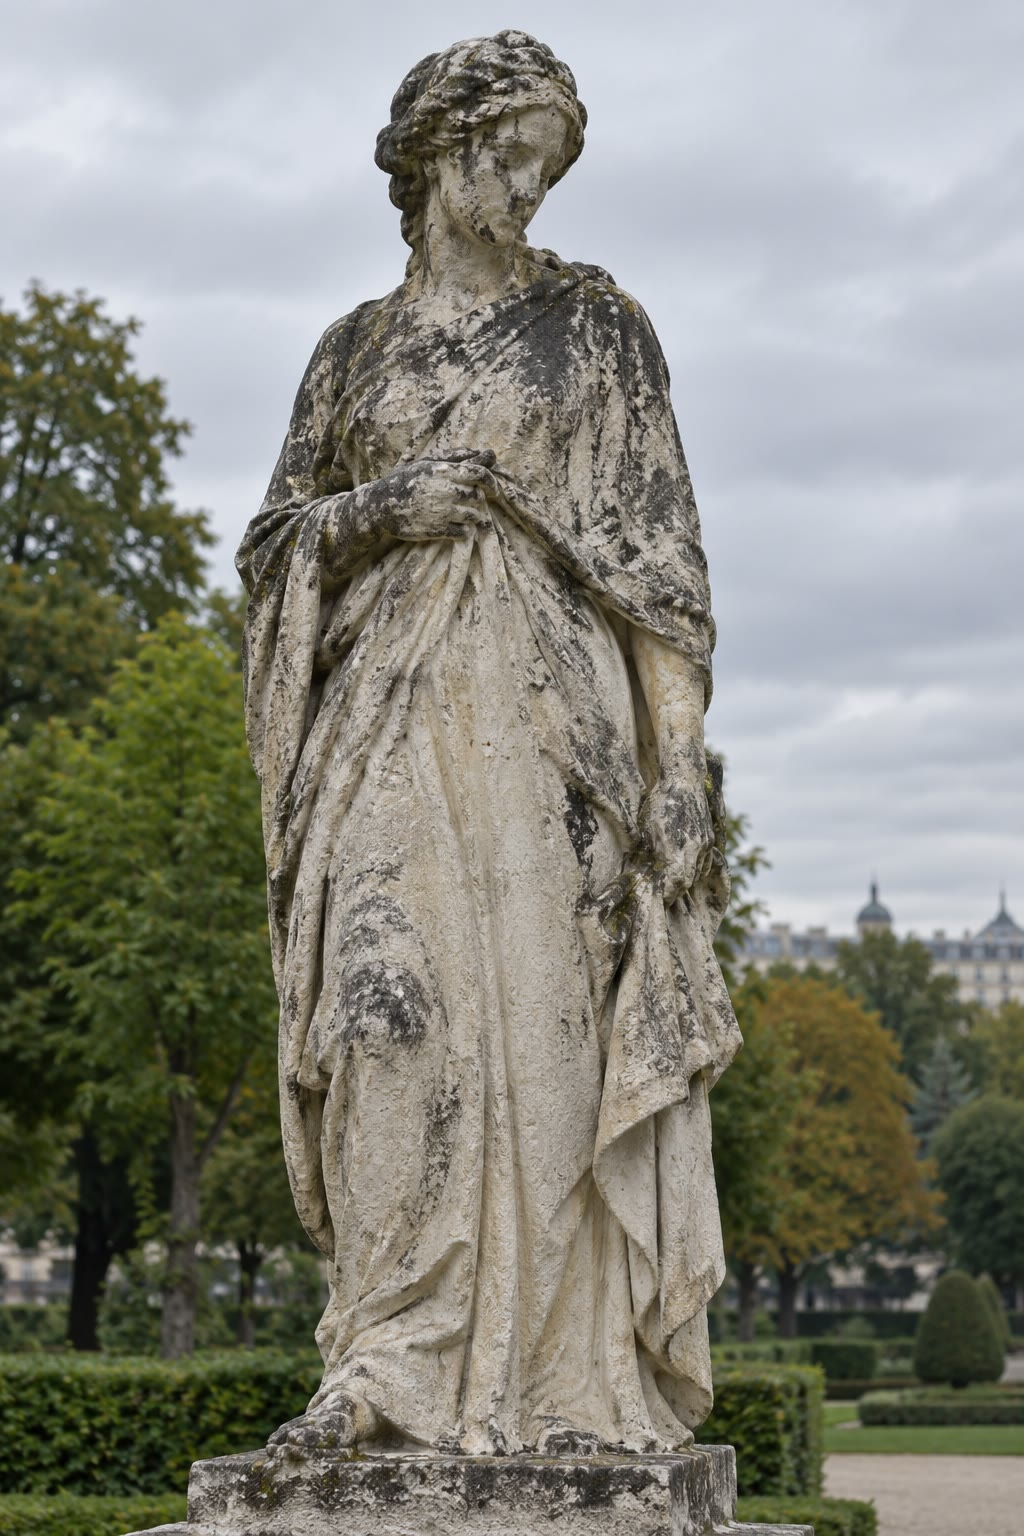
\includegraphics[width=0.42\linewidth,height=6cm,keepaspectratio]{images/book1/ai/g12-weathered-statue.jpg}

{\small Una estatua de caliza desgastada por la lluvia: una reacción que
tarda siglos.}
\end{omfigure}

\section{Velocidades de desaparición y de aparición}

\begin{definition}[Velocidad de desaparición, velocidad de aparición]\label{def:g12:reaction-rates:rate}
En una disolución de volumen constante, la \emph{velocidad de desaparición}\index{velocidad de desaparicion@velocidad de desaparición}
de un \omterm{def:g7:chemical-reactions:reactant}{reactivo} A en el instante $t$ es
\[
  v_A(t) = -\frac{d[\ce{A}]}{dt},
\]
y la \emph{velocidad de aparición}\index{velocidad de aparicion@velocidad de aparición} de un
producto P es $v_P(t) = \dfrac{d[\ce{P}]}{dt}$. Ambas son positivas, en
\si{mol.L^{-1}.min^{-1}} (o por segundo).
\end{definition}


\begin{method}[Leer una velocidad en una tangente]\label{met:g12:reaction-rates:tangent}
\begin{enumerate}
  \item En la curva de $[\ce{A}]$ en función de $t$, traza la tangente en
        el instante elegido.
  \item Lee dos puntos alejados de la tangente y calcula su pendiente,
        $\Delta[\ce{A}] / \Delta t$.
  \item La \omterm{def:g12:reaction-rates:rate}{velocidad de desaparición} es la opuesta de esta pendiente
        (para un producto, la propia pendiente).
\end{enumerate}
\end{method}

\begin{omfigure}
\begin{tikzpicture}
\begin{axis}[width=0.8\linewidth, height=6.4cm, xmin=0, xmax=60, ymin=0,
    ymax=11, xlabel={$t$ (\si{min})}, ylabel={$[\ce{A}]$ (\si{mmol/L})},
    axis lines*=left, ymajorgrids, xmajorgrids, grid style={gray!20},
    tick label style={font=\small}, label style={font=\small},
    legend style={font=\small, at={(0.98,0.97)}, anchor=north east,
    draw=none, fill=white}, legend cell align=left]
  \addplot[very thick, omDef] table[x=t, y=A1] {figdata/out/grade-12-reaction-rates-a.dat};
  \addplot[very thick, omThm] table[x=t, y=A2] {figdata/out/grade-12-reaction-rates-a.dat};
  \addplot[thick, dashed, omProp, restrict y to domain=0:11] table[x=t, y=tangent]
    {figdata/out/grade-12-reaction-rates-a.dat};
  \legend{$k = \qty{0.050}{min^{-1}}$, $k = \qty{0.100}{min^{-1}}$ (más caliente),
    tangente en $t = 0$}
  \addplot[densely dotted, black!60] coordinates {(0,5) (13.86,5) (13.86,0)};
  \addplot[densely dotted, black!60] coordinates {(6.93,5) (6.93,0)};
  \node[font=\small, anchor=south west] at (axis cs:14.6,5.4) {$t_{1/2} = \qty{13.9}{min}$};
  \node[font=\small, anchor=south east] at (axis cs:6.7,0.2) {\qty{6.9}{min}};
\end{axis}
\end{tikzpicture}

{\small La concentración de un \omterm{def:g7:chemical-reactions:reactant}{reactivo} A en función del tiempo, para la
misma \omterm{def:g12:reaction-rates:first-order}{reacción de primer orden} a dos temperaturas. La tangente en
$t = 0$ (discontinua) da la velocidad inicial; las líneas de puntos
marcan los \omterm{def:g12:reaction-rates:half-life}{tiempos de semirreacción}.}
\end{omfigure}

\begin{example}[La velocidad inicial]\label{ex:g12:reaction-rates:initial}
En la curva azul, la tangente en $t = 0$ va de \qty{10.0}{mmol/L} en
$t = 0$ a $0$ en $t = \qty{20}{min}$: su pendiente es
$-10.0/20 = \qty{-0.50}{mmol.L^{-1}.min^{-1}}$, así que la velocidad
inicial de desaparición es \qty{0.50}{mmol.L^{-1}.min^{-1}}. Más tarde la
curva se aplana y la velocidad disminuye: la reacción se frena a medida
que A se consume.
\end{example}

\section{Reacciones de primer orden}

\begin{definition}[Reacción de primer orden, constante de velocidad]\label{def:g12:reaction-rates:first-order}
Una reacción es una \emph{reacción de primer orden}\index{reaccion de primer orden@reacción de primer orden}
respecto a A si su \omterm{def:g12:reaction-rates:rate}{velocidad de desaparición} es proporcional a la
concentración de A en todo instante:
\[
  -\frac{d[\ce{A}]}{dt} = k\,[\ce{A}] .
\]
La constante positiva $k$, en \si{min^{-1}} o \si{s^{-1}}, es la
\emph{constante de velocidad}\index{constante de velocidad}; depende de la
temperatura.
\end{definition}

\begin{proposition}[Decrecimiento exponencial]\label{prop:g12:reaction-rates:exponential}
Para una \omterm{def:g12:reaction-rates:first-order}{reacción de primer orden} con concentración inicial $[\ce{A}]_0$,
\[
  [\ce{A}](t) = [\ce{A}]_0\, e^{-kt} .
\]
\end{proposition}

\begin{proof}
La función $f(t) = [\ce{A}]_0 e^{-kt}$ tiene por derivada
$f'(t) = -k [\ce{A}]_0 e^{-kt} = -k f(t)$, así que cumple la ecuación de
velocidad, y $f(0) = [\ce{A}]_0$. Que sea la única función así se admite
aquí (se demuestra en matemáticas, para las ecuaciones $y' = ay$).
\end{proof}

\begin{method}[Comprobar el primer orden]\label{met:g12:reaction-rates:test}
\begin{enumerate}
  \item A partir de las medidas, calcula $\ln [\ce{A}]$ (o $\ln A$ para
        una \omterm{def:g11:absorbance:absorbance}{absorbancia} proporcional a $[\ce{A}]$) en cada instante.
  \item Representa $\ln[\ce{A}]$ en función de $t$: como
        $\ln[\ce{A}] = \ln[\ce{A}]_0 - kt$, los puntos están alineados si y
        solo si la reacción es de primer orden.
  \item La pendiente de la recta es $-k$.
\end{enumerate}
\end{method}

\section{Tiempo de semirreacción}

\begin{definition}[Tiempo de semirreacción]\label{def:g12:reaction-rates:half-life}
El \emph{tiempo de semirreacción}\index{tiempo de semirreaccion@tiempo de semirreacción}
$t_{1/2}$ de una reacción es el tiempo que tarda la concentración del
\omterm{def:g10:reaction-progress-table:limiting}{reactivo limitante} en bajar a la mitad de su valor inicial.
\end{definition}

\begin{proposition}[Tiempo de semirreacción de una reacción de primer orden]\label{prop:g12:reaction-rates:half-life}
Para una \omterm{def:g12:reaction-rates:first-order}{reacción de primer orden},
\[
  t_{1/2} = \frac{\ln 2}{k},
\]
sea cual sea la concentración inicial; al cabo de $n$ \omterm{def:g12:reaction-rates:half-life}{tiempos de
semirreacción}, la concentración se ha dividido por $2^n$.
\end{proposition}

\begin{proof}
$[\ce{A}]_0 e^{-k t_{1/2}} = [\ce{A}]_0 / 2$ da $e^{-k t_{1/2}} = 1/2$,
así que $k t_{1/2} = \ln 2$. Cada nuevo \omterm{def:g12:reaction-rates:half-life}{tiempo de semirreacción} vuelve a
multiplicar la concentración por $e^{-k t_{1/2}} = 1/2$.
\end{proof}


\begin{example}[Leer los tiempos de semirreacción]\label{ex:g12:reaction-rates:half-lives}
Para $k = \qty{0.050}{min^{-1}}$, $t_{1/2} = 0.693 / 0.050 =
\qty{13.9}{min}$: la concentración baja de 10.0 a 5.0, luego a 2.5 y
luego a \qty{1.25}{mmol/L} a los 13.9, 27.7 y \qty{41.6}{min}. El ensayo
más caliente, con una $k$ el doble de grande, tiene un \omterm{def:g12:reaction-rates:half-life}{tiempo de
semirreacción} la mitad, \qty{6.9}{min}, como muestra la figura.
\end{example}

\begin{remark}[Semividas en otros ámbitos]\label{rem:g12:reaction-rates:radioactive}
En física se usa la misma idea, con el nombre de periodo de
semidesintegración, para los \omterm{def:g9:inside-the-atom:nucleus}{núcleos} radiactivos, cuyo número disminuye
de la misma forma exponencial: una desintegración radiactiva se comporta
como una \omterm{def:g12:reaction-rates:first-order}{reacción de primer orden}. El libro de física la estudia.
\end{remark}

\begin{omfigure}
\begin{minipage}{0.49\linewidth}
\begin{tikzpicture}
\begin{axis}[width=\linewidth, height=5.4cm, xmin=0, xmax=26, ymin=0,
    ymax=0.85, xlabel={$t$ (\si{min})}, ylabel={absorbancia $A$},
    axis lines*=left, ymajorgrids, grid style={gray!20},
    tick label style={font=\scriptsize}, label style={font=\small}]
  \addplot[only marks, mark=*, mark size=1.8pt, omDef] table[x=t, y=A]
    {figdata/out/grade-12-reaction-rates-b.dat};
  \addplot[thick, omProp, domain=0:26, samples=60] {0.8*exp(-0.11552*x)};
\end{axis}
\end{tikzpicture}
\end{minipage}\hfill
\begin{minipage}{0.49\linewidth}
\begin{tikzpicture}
\begin{axis}[width=\linewidth, height=5.4cm, xmin=0, xmax=26, ymin=-3.4,
    ymax=0, xlabel={$t$ (\si{min})}, ylabel={$\ln A$}, axis lines*=left,
    ymajorgrids, grid style={gray!20}, tick label style={font=\scriptsize},
    label style={font=\small}]
  \addplot[only marks, mark=*, mark size=1.8pt, omDef] table[x=t, y=lnA]
    {figdata/out/grade-12-reaction-rates-b.dat};
  \addplot[thick, omProp, domain=0:26] {-0.2231-0.11552*x};
\end{axis}
\end{tikzpicture}
\end{minipage}

{\small La decoloración del violeta cristal en \omterm{def:g9:acids-bases-ph:acidic}{disolución básica} (datos
del problema de fin de semana). Izquierda: la \omterm{def:g11:absorbance:absorbance}{absorbancia} disminuye
siguiendo una exponencial. Derecha: $\ln A$ en función de $t$ es una
recta de pendiente $-\qty{0.116}{min^{-1}}$: la reacción es de primer
orden respecto al colorante.}
\end{omfigure}

\section{Ejercicios}

\begin{exercise}[$\star$]\label{exo:g12:reaction-rates:1}
Nombra el \omterm{def:g12:reaction-rates:kinetic-factor}{factor cinético} que actúa en cada caso: una nevera conserva los
alimentos; el azúcar en polvo se \omterm{def:g2:mixing-and-dissolving:dissolve}{disuelve} más deprisa que un terrón; un
ácido más concentrado ataca el cinc más deprisa; una manzana cortada se
oscurece más deprisa en verano.
\end{exercise}

\begin{exercise}[$\star$]\label{exo:g12:reaction-rates:2}
Lee en la figura de $[\ce{A}]$ en función del tiempo el \omterm{def:g12:reaction-rates:half-life}{tiempo de
semirreacción} de cada ensayo. ¿Cuánto vale $[\ce{A}]$ en la curva azul
al cabo de dos \omterm{def:g12:reaction-rates:half-life}{tiempos de semirreacción}?
\end{exercise}

\begin{exercise}[$\star$]\label{exo:g12:reaction-rates:3}
Una tangente a la curva de un producto trazada en $t = \qty{5}{min}$ pasa
por $(0, \qty{1.0}{mmol/L})$ y $(\qty{10}{min}, \qty{5.0}{mmol/L})$.
¿Cuál es la \omterm{def:g12:reaction-rates:rate}{velocidad de aparición} del producto a los \qty{5}{min}?
\end{exercise}

\begin{exercise}[$\star$]\label{exo:g12:reaction-rates:4}
¿Por qué se vierte una muestra en agua helada antes de valorarla? ¿Por
qué hay que anotar el instante de la muestra cuando se vierte, y no
cuando se valora?
\end{exercise}

\begin{exercise}[$\star$]\label{exo:g12:reaction-rates:5}
Una \omterm{def:g12:reaction-rates:first-order}{reacción de primer orden} tiene un \omterm{def:g12:reaction-rates:half-life}{tiempo de semirreacción} de
\qty{10}{min}. ¿Qué fracción del \omterm{def:g7:chemical-reactions:reactant}{reactivo} queda al cabo de
\qty{30}{min}? ¿Y al cabo de \qty{1}{h}?
\end{exercise}

\begin{exercise}[$\star\star$]\label{exo:g12:reaction-rates:6}
Concentraciones de un \omterm{def:g7:chemical-reactions:reactant}{reactivo}, en \si{mmol/L}: 8.00 a \qty{0}{min},
5.66 a \qty{5}{min}, 4.00 a \qty{10}{min}, 2.83 a \qty{15}{min}, 2.00 a
\qty{20}{min}. Calcula $\ln[\ce{A}]$ en cada instante y demuestra que la
reacción es de primer orden. Halla $k$ y el \omterm{def:g12:reaction-rates:half-life}{tiempo de semirreacción}.
\end{exercise}

\begin{exercise}[$\star\star$]\label{exo:g12:reaction-rates:7}
Una \omterm{def:g12:reaction-rates:first-order}{reacción de primer orden} tiene $t_{1/2} = \qty{25}{s}$. Calcula $k$.
\end{exercise}

\begin{exercise}[$\star\star$]\label{exo:g12:reaction-rates:8}
Para $[\ce{A}]_0 = \qty{0.100}{mol/L}$ y $k = \qty{0.020}{min^{-1}}$,
calcula $[\ce{A}]$ al cabo de 10, 30 y \qty{100}{min}.
\end{exercise}

\begin{exercise}[$\star\star$]\label{exo:g12:reaction-rates:9}
En la figura de $[\ce{A}]$ en función del tiempo, estima la pendiente de
la curva azul en $t = \qty{13.9}{min}$ (traza una tangente) y compárala
con $-k[\ce{A}]$ en ese instante.
\end{exercise}

\begin{exercise}[$\star\star$]\label{exo:g12:reaction-rates:10}
El yodo \ce{I2}, de color pardo, se forma lentamente en una disolución
incolora. La \omterm{def:g11:absorbance:absorbance}{absorbancia} sube de 0 hacia 0.60. Explica por qué la
\omterm{def:g11:absorbance:absorbance}{absorbancia} sirve para seguir $[\ce{I2}]$, y cómo se lee en la curva de
$A$ en función de $t$ la \omterm{def:g12:reaction-rates:rate}{velocidad de aparición} en un instante dado.
\end{exercise}

\begin{exercise}[$\star\star$]\label{exo:g12:reaction-rates:11}
Dos ensayos de la misma reacción empiezan con $[\ce{A}]_0 = 10$ y
\qty{20}{mmol/L}. Si la reacción es de primer orden, compara sus
velocidades iniciales y sus \omterm{def:g12:reaction-rates:half-life}{tiempos de semirreacción}.
\end{exercise}

\begin{exercise}[$\star\star\star$]\label{exo:g12:reaction-rates:12}
¿Cuántos \omterm{def:g12:reaction-rates:half-life}{tiempos de semirreacción} tarda una \omterm{def:g12:reaction-rates:first-order}{reacción de primer orden} en
reducir su \omterm{def:g7:chemical-reactions:reactant}{reactivo} al \qty{1}{\percent}? ¿Y al \qty{0.1}{\percent}? Da
la fórmula general del tiempo necesario para bajar a una fracción $f$.
\end{exercise}

\begin{exercise}[$\star\star\star$]\label{exo:g12:reaction-rates:13}
Una reacción tiene $k = \qty{0.050}{min^{-1}}$ a \qty{20}{\celsius} y
$k = \qty{0.100}{min^{-1}}$ a \qty{30}{\celsius}. ¿Cuánto tarda en
consumir el \qty{90}{\percent} del \omterm{def:g7:chemical-reactions:reactant}{reactivo} a cada temperatura? Una regla
práctica habitual dice que la velocidad se duplica cada
\qty{10}{\celsius}: ¿la cumple esta reacción?
\end{exercise}

\begin{exercise}[$\star\star\star$]\label{exo:g12:reaction-rates:14}
Se bloquea una muestra vertiendo \qty{5.0}{mL} en \qty{45}{mL} de agua
helada. Da dos razones por las que la reacción se vuelve mucho más
lenta. Si la reacción es de primer orden respecto a cada uno de dos
\omterm{def:g7:chemical-reactions:reactant}{reactivos}, ¿por qué factor divide la velocidad la \omterm{def:g10:concentration-and-dilution:dilution}{dilución} por sí sola?
\end{exercise}

\begin{exercise}[$\star\star\star$]\label{exo:g12:reaction-rates:15}
Demuestra, derivando, que la \omterm{def:g12:reaction-rates:rate}{velocidad de desaparición} de una \omterm{def:g12:reaction-rates:first-order}{reacción
de primer orden} es a su vez una función exponencial del tiempo,
$v(t) = k[\ce{A}]_0 e^{-kt}$. ¿Cuál es la velocidad inicial? ¿Al cabo de
cuánto tiempo es la velocidad la mitad de la inicial?
\end{exercise}

\section{Problema: el colorante que se desvanece}

\begin{problem}[{Problema de fin de semana --- violeta cristal decolorado por iones
hidróxido: ¿cuánto tarda el color en desaparecer casi por completo?}]
\label{pb:g12:reaction-rates:1}
El colorante violeta cristal reacciona con los \omterm{def:g9:ions:ion}{iones} hidróxido y da un
producto incoloro. Con un gran exceso de hidróxido, la velocidad solo
depende de la concentración del colorante. La \omterm{def:g11:absorbance:absorbance}{absorbancia} de la
disolución se registra a la longitud de onda en la que el colorante
absorbe más:
\begin{center}
\small
\begin{tabular}{l*{10}{c}}
\hline
$t$ (\si{min}) & 0 & 2 & 4 & 6 & 8 & 10 & 12 & 15 & 20 & 25 \\
$A$ & 0.800 & 0.639 & 0.501 & 0.402 & 0.315 & 0.255 & 0.199 & 0.143 &
0.078 & 0.046 \\
\hline
\end{tabular}
\end{center}

\medskip
\noindent\textbf{Parte I --- \omterm{def:g11:absorbance:absorbance}{Absorbancia} y concentración.}
\begin{enumerate}
  \item ¿Por qué la \omterm{def:g11:absorbance:absorbance}{absorbancia} es proporcional a la concentración del
        colorante? ¿Qué condición debe cumplir la disolución?
  \item ¿Por qué el producto, incoloro, no se ve a esta longitud de onda?
  \item ¿Por qué se usa el hidróxido en gran exceso?
  \item ¿Qué se leería en el espectrofotómetro al final de la reacción?
\end{enumerate}

\medskip
\noindent\textbf{Parte II --- ¿Es de primer orden?}
\begin{enumerate}[resume]
  \item Lee directamente en la tabla el \omterm{def:g12:reaction-rates:half-life}{tiempo de semirreacción}.
  \item Comprueba que es el mismo de $t = 6$ a $t = 12$ min.
  \item Calcula $\ln A$ en cada instante.
  \item Representa $\ln A$ en función de $t$ (o usa la figura del
        capítulo). ¿Qué observas? Concluye.
  \item Calcula la pendiente a partir de los puntos de 0 y de
        \qty{20}{min}.
\end{enumerate}

\medskip
\noindent\textbf{Parte III --- La \omterm{def:g12:reaction-rates:first-order}{constante de velocidad}.}
\begin{enumerate}[resume]
  \item Deduce $k$.
  \item Calcula el \omterm{def:g12:reaction-rates:half-life}{tiempo de semirreacción} a partir de $k$ y compáralo
        con la pregunta 5.
  \item Calcula la velocidad inicial de desaparición del colorante,
        expresada como velocidad de disminución de la \omterm{def:g11:absorbance:absorbance}{absorbancia}.
  \item ¿Cuál sería el \omterm{def:g12:reaction-rates:half-life}{tiempo de semirreacción} si la \omterm{def:g11:absorbance:absorbance}{absorbancia} inicial
        fuera 0.400?
\end{enumerate}

\medskip
\noindent\textbf{Parte IV --- Predicción.}
\begin{enumerate}[resume]
  \item Predice la \omterm{def:g11:absorbance:absorbance}{absorbancia} a los \qty{30}{min}.
  \item ¿En qué instante baja la \omterm{def:g11:absorbance:absorbance}{absorbancia} a 0.008, el \qty{1}{\percent}
        de su valor inicial?
  \item ¿A cuántos \omterm{def:g12:reaction-rates:half-life}{tiempos de semirreacción} corresponde?
  \item El ojo deja de ver el color por debajo de $A = 0.010$
        aproximadamente. ¿Cuándo parece incolora la disolución?
  \item Se repite el experimento \qty{10}{\celsius} más caliente y el
        \omterm{def:g12:reaction-rates:half-life}{tiempo de semirreacción} pasa a ser de \qty{3.0}{min}. ¿Cuándo se
        alcanza el \qty{1}{\percent}?
  \item Da la respuesta final: ¿cuántos \omterm{def:g12:reaction-rates:half-life}{tiempos de semirreacción} tarda
        el color en bajar al \qty{1}{\percent} de su valor inicial, y
        cuántos minutos son aquí?
\end{enumerate}
\end{problem}
